\documentclass[tikz,border=10pt]{standalone}
\usepackage{tikz}
\usetikzlibrary{arrows.meta,positioning,calc,shapes.geometric}

\begin{document}
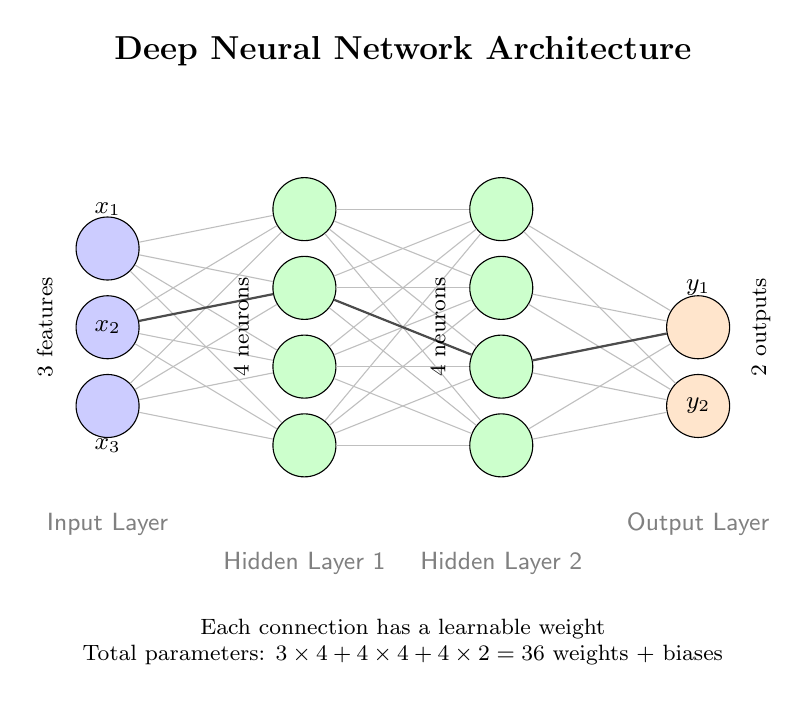
\begin{tikzpicture}[
    neuron/.style={circle, draw, fill=blue!20, minimum size=0.8cm},
    hidden/.style={circle, draw, fill=green!20, minimum size=0.8cm},
    output/.style={circle, draw, fill=orange!20, minimum size=0.8cm},
    layer_label/.style={font=\small\sffamily, text=gray},
    connection/.style={draw, gray!50},
    thick_connection/.style={draw, black!70, thick}
]

% Define layer positions
\def\inputlayer{0}
\def\hiddenlayerone{2.5}
\def\hiddenlayertwo{5}
\def\outputlayer{7.5}

% Title
\node[font=\large\bfseries] at (3.75, 4) {Deep Neural Network Architecture};

% Input layer
\foreach \i in {1,2,3} {
    \node[neuron] (input\i) at (\inputlayer, {2.5-\i}) {};
}
\node[layer_label] at (\inputlayer, -2) {Input Layer};
\node[font=\small] at (\inputlayer, 2) {$x_1$};
\node[font=\small] at (\inputlayer, 0.5) {$x_2$};
\node[font=\small] at (\inputlayer, -1) {$x_3$};

% First hidden layer
\foreach \i in {1,2,3,4} {
    \node[hidden] (hidden1\i) at (\hiddenlayerone, {3-\i}) {};
}
\node[layer_label] at (\hiddenlayerone, -2.5) {Hidden Layer 1};

% Second hidden layer
\foreach \i in {1,2,3,4} {
    \node[hidden] (hidden2\i) at (\hiddenlayertwo, {3-\i}) {};
}
\node[layer_label] at (\hiddenlayertwo, -2.5) {Hidden Layer 2};

% Output layer
\foreach \i in {1,2} {
    \node[output] (output\i) at (\outputlayer, {1.5-\i}) {};
}
\node[layer_label] at (\outputlayer, -2) {Output Layer};
\node[font=\small] at (\outputlayer, 1) {$y_1$};
\node[font=\small] at (\outputlayer, -0.5) {$y_2$};

% Connections - Input to Hidden1
\foreach \i in {1,2,3} {
    \foreach \j in {1,2,3,4} {
        \draw[connection] (input\i) -- (hidden1\j);
    }
}

% Connections - Hidden1 to Hidden2
\foreach \i in {1,2,3,4} {
    \foreach \j in {1,2,3,4} {
        \draw[connection] (hidden1\i) -- (hidden2\j);
    }
}

% Connections - Hidden2 to Output
\foreach \i in {1,2,3,4} {
    \foreach \j in {1,2} {
        \draw[connection] (hidden2\i) -- (output\j);
    }
}

% Highlight one path
\draw[thick_connection] (input2) -- (hidden12);
\draw[thick_connection] (hidden12) -- (hidden23);
\draw[thick_connection] (hidden23) -- (output1);

% Annotations
\node[align=center, font=\footnotesize] at (3.75, -3.5) {
Each connection has a learnable weight\\
Total parameters: $3 \times 4 + 4 \times 4 + 4 \times 2 = 36$ weights + biases
};

% Dimension labels
\node[font=\footnotesize, rotate=90] at (-0.8, 0.5) {3 features};
\node[font=\footnotesize, rotate=90] at (1.7, 0.5) {4 neurons};
\node[font=\footnotesize, rotate=90] at (4.2, 0.5) {4 neurons};
\node[font=\footnotesize, rotate=90] at (8.3, 0.5) {2 outputs};

\end{tikzpicture}
\end{document}